% Arara build configuration:
% arara: pdflatex: {synctex: on, shell: true}
% arara: bibtex
% nomencl: {style: 'nomencl'}
% pdflatex: { synctex: on }
% pdflatex: { synctex: on }

%\includeonly{chap/legdesign}
\documentclass[listof=totoc,bibliography=totoc,11pt,twoside,BCOR=12mm,DIV=11]{scrbook}
\linespread{1.25}

%\usepackage{showframe}  %to show typing area, header, footer, margins

\usepackage[english]{babel}
\usepackage{amsmath}
\usepackage{amsfonts}
\usepackage{amssymb}
\usepackage[T1]{fontenc}
\usepackage{charter} %set font
%\setkomafont{disposition}{\bfseries}
\addtokomafont{chapter}{\Huge} %set font parameter
\addtokomafont{section}{\huge} %set font parameter
\addtokomafont{subsection}{\LARGE} %set font parameter
\addtokomafont{subsubsection}{\Large} %set font parameter

%\usepackage[headsepline,footsepline]{scrpage2}
%\pagestyle{scrheadings}
%\setheadsepline{3pt}

%\usepackage[round,mcite]{natbib} %bibliography

\usepackage[hidelinks]{hyperref} %hyperlinks in pdf

\usepackage{blindtext}  %to create a dummy document
\usepackage{lipsum} %content filler

\usepackage{graphicx}
\DeclareGraphicsExtensions{.pdf,.png,.jpg,.eps} %images without extension
\usepackage{subfig} %use subfigure configurations

\usepackage{textcomp} %copyright symbols

%Nomenclature
\usepackage[intoc]{nomencl}
\makenomenclature

% customize dictum format:
\setkomafont{dictumtext}{\itshape\small}
\setkomafont{dictumauthor}{\normalfont}
\renewcommand*\dictumwidth{\linewidth}
\renewcommand*\dictumauthorformat[1]{--- #1}
\renewcommand*\dictumrule{}

\begin{document}

\frontmatter
\titlehead{
\begin{center}
\includegraphics[width = 0.35\textwidth]{images/uctround.png}
\end{center}
}
\subject{Faculty of Engineering and the Built Environment \\
Department of Electrical Engineering \\}
\title{{Hopping Control of a Single Leg Robot}}
\subtitle{Prepared for Dr. Amir Patel.
\linebreak
Submitted to the Department of Electrical Engineering\\at the University of Cape Town in partial
fulfilment\\ of the academic requirements\\for a Bachelor of Science (Eng.) degree in Mechatronics.
}
\author{Benjamin Scholtz}
%\date{date}
\publishers{\textbf{Keywords:} robotics, virtual model, compliance control, force control, mechatronics}
\dedication{To all the people that helped me jump!\\ \medskip \includegraphics[width = 0.4\textwidth]{images/leg-mount.png}}
\maketitle
\chapter{Declaration}
\begin{enumerate}
\item I know that plagiarism is wrong. Plagiarism is to use another's work and pretend that it
is one's own.
\item I have used the IEEE convention for citation and referencing. Each contribution to, and
quotation in, this final year project report from the work(s) of other people, has been attributed and has been cited and referenced.
\item This final year project report is my own work.
\item I have not allowed, and will not allow, anyone to copy my work with the intention of passing it off as their own work or part thereof.
\end{enumerate}

\bigskip

\noindent
Name: Benjamin Scholtz \\
Signature: \underline{\hspace{3cm}} \\
Date: \today \\
\chapter{Abstract}

A vertically constrained direct drive robotic leg platform was modelled, simulated, designed, built, and tested in order to better understand rapid acceleration control. The research was performed to investigate the following questions: \textbf{Is a virtual model a suitable replacement for accurate dynamic modelling in complex robotic topologies? Can high fidelity force control be effectively implemented without using force feedback? Is a virtual compliance control system effective in handling high speed impacts and executing rapid acceleration manoeuvres?} The dynamic model of the robot is complex, instead a virtual model uses simulations of components placed on the body of the robot to generate the desired end effector force response. The end effector was virtually modelled in the polar coordinate system as a radial and torsional series spring-damper. The desired virtual model motor torques were generated using the Jacobian kinematic mapping. Proprioceptive force control was possible due to the transparent coupling between the direct drive actuator and end effector. An iterative hardware and software design process was used to enable effective robotic testing - both an embedded communication and control system, and a GUI, were developed for the platform. Experiments were performed in virtual model spring-damping, impact absorption, trajectory tracking, force control, and current control. Jump tests were performed investigating robustness, repeatability, and rapid acceleration control. Force control and virtual model fidelity were verified by critically analysing both theoretical simulated responses and practical data. The robot generated an energy of $3.9\ J/kg$ with a maximum hopping height of $0.4\ m$, comparing well to the current state of the art. Robust hopping control was achieved with an $8.57\%$ mean time shift and a negligible mean peak force deviation over 7 consecutive jumps. A robust robotic platform was successfully developed that enabled high fidelity force control using a virtual compliance model. The research contributed a platform and control framework that can be effectively used in future rapid acceleration research in the UCT Mechatronics Lab.


\chapter{Acknowledgements}
I'd like to thank my friends in the lab, some of whom were responsible for convincing me to take on this daunting project! Craig Burden, Gareth Callanan, Roberto Aldera, Munnawar Tayob, Michael Evans and Brad Stocks. 

All the post graduate researchers in the lab (from fourth year number... 3?) -- thank you for the endless support and missions to the UCT pub! I'd specifically like to thank Callen Fisher for the assistance, sharp mind, and sometimes harsh words to set us on track without hesitation! 

To the mechatronics lab squash team -- I hope to be able to play against you all again, I restrung my racquet just for that chance... Callen (still to beat), Stacey, Neil, Arnold, Givs, Tinashe (most improved and serious comeback!), Robyn.

Ben Bingham and Luke Bell -- your contribution to the project was a great kick-start that helped avoid a lot of trouble! Thank you for being quick to help.

Brendan Daniels and Justin Pead -- you were there day in and out, dealing with that pesky laser cutter, providing handfuls of components, defusing near blown LiPos, and providing your time to 3D print parts for Baleka.

My family -- for all the tea ferried up to my room, dealing with my hermit like habits in the final stretch, and the care!

Last and certainly not least, my supervisor, Dr. Amir Patel -- your guidance was strong, and your words and endless enthusiasm gave confidence when needed most! The project was a daunting task and you helped define my research vision.

\chapter{Terms of Reference}
\lipsum

\textsf{\tableofcontents}
%\tableofcontents

\listoffigures
\listoftables
\renewcommand\listoflistingscaption{List of Source Codes}
\listoflistings

%\printnomenclature

\mainmatter
%ch01: Introduction
%ch02: Literature Review
%ch03: Project Plan and Methodology
%ch04: Theory Development
%ch05: System Modelling and Simulation
%ch06: Conclusions
%ch07: Recommendations and Future Work

%\autoref{chap:intro}

\setchapterpreamble[uc][.75\textwidth]{%
\dictum[Lewis Carroll, \textit{Alice in Wonderland}]{%
``Begin at the beginning,'' the King said, gravely, ``and go on till you
come to an end; then stop.''}\vskip1em}

\chapter{Introduction}
\label{chap:intro}

With a hop, skip, and a jump -- the journey begins!

\section{Background}
\section{Objectives of the Study}
\subsection{Problems to be Investigated}
\subsection{Research Questions}
\subsection{Purpose of the Study}
\section{Scope and Limitations}
\section{Plan of Development}
\chapter{Literature Review}

\section{Introduction}

Would be robotics engineers take their inspiration from popular culture with The Iron Giant (\cref{fig:the-iron-giant-1999}) and B.E.N. (\cref{fig:BEN-treasure-island-2002}) fresh in mind. The Rising Sun included robots developed by Marc Raibert (\cref{fig:rising-sun}), founder of the CMU (now MIT) Leg Laboratory, who pioneered self-balancing dynamic control of hopping robots. 

Robotics turned towards pairing complex dynamic responses with simple control systems when Marc Raibert developed the dynamically stable Planar One-Leg Hopper in 1980. Development continued until the Atlas humanoid robot (2013) of Boston Dynamics achieved human like static stability and the Cheetah Robot V2 (2015) of MIT Biomimetics achieved lifelike legged manoeuvres. 

The literature covered in this review will lead us from the natural locomotion of Kangaroos to the supernatural motion of complex legged machines. From one-legged hoppers to Baleka like forms, these robots will each be critically discussed to draw parallels between the current state of the art and Baleka as well as discovering the contribution that Baleka can make to current research. The art of force control will be touched on before the applications of such control will be seen in industry. Modelling, control, and actuation methods will be investigated and considered for use on Baleka.

\begin{figure}
\centering
\subfloat[][The Iron Giant (1999).]{
\includegraphics[width=0.6\textwidth]{images/literature/the-iron-giant-1999.jpg} 
\label{fig:the-iron-giant-1999}
}

\subfloat[][Rising Sun (1993).]{
\includegraphics[width=0.3\textwidth]{images/literature/rising-sun.jpg} 
\label{fig:rising-sun}
}
\subfloat[][Treasure Planet (2002).]{
\includegraphics[width=0.3\textwidth]{images/literature/BEN-treasure-island-2002.jpg} 
\label{fig:BEN-treasure-island-2002}
}
\caption{Humanoid robots in popular culture.}
\end{figure}

\section{Legged Locomotion in Nature}
\label{sec:Legged Locomotion in Nature}

The study in \cite{Farley1996} modelled the human leg as a spring loaded inverted pendulum, as seen in \cref{fig:Model of a human leg}, and found that it described the mechanics of biological running well. The study concluded that the biological leg spring has a higher spring constant for higher stride frequencies.\cite{Farley1996} A stiffer spring is able to absorb and impart more energy over the course of a stride, thus enabling a higher stride frequency. The Baleka leg is limited to movement in a single vertical axis, but the virtual spring stiffness should have the same effect on energy transfer as found in this study -- a transfer of energy from spring energy to peak potential energy at the highest point of the jump.

When animals run, they use a hopping movement. This hopping movement is defined by limited contact with the ground with phases of mid-air motion. Cavagna et al found that they use musculoskeletal springs to store and return elastic energy.\cite{Farley1996} This storage and release of elastic energy is the principal on which Baleka's control system will be developed - by controlling the theoretical transfer of energy between jump phases one should be able to achieve height control and impact absorption, as discussed in \cref{chap:Dynamic Modelling}.

Farley et al determined that the leg spring stiffness of animals remains the same at all speeds, this shows a clear natural design element that serves a purpose in energy transfer and control during running.\cite{Farley1996}

The study in \cite{Alexander2009} found that the hopping motion of a Kangaroo is split into two phases, a contact phase and a floating phase. The phases were investigated using kinetic and potential energy, where it was found that at high speed there were more fluctations in kinetic energy and less in potential energy - this means that work is being done and energy is being added to the system through actuation of the Kangaroo's tendons.\cite{Alexander2009} In a simple hopping motion on the other hand, as is the case with Baleka, the majority of the kinetic energy should be efficiently transferred to potential energy.

\cite{Alexander2009} also mathematically derives the energy relation of launch and impact on the Kangaroo's forward motion. It was found that the line of action of the force exerted by a Kangaroo on the ground always passes through the center of mass.\cite{Alexander2009} This is useful theory in the case of Baleka being modelled as a spring-damper mass system, as it confirms the assumption that the force input to the system can be simplified as a gravitational force acting on the center of mass. 

\begin{figure}
\centering
\includegraphics[width=0.4\textwidth]{images/literature/human-leg-spring-model} 
\caption{Model of a human leg as an inverted spring mass system - Farley and Gonzalez (1996).\cite{Farley1996}}
\label{fig:Model of a human leg}
\end{figure}

\section{State of the Art in Legged Robotics}

The development of dynamic hopping control in robots started under Marc Raibert's guidance at the CMU Leg Laboratory in 1980. He then moved the lab to the MIT Leg Laboratory and founded Boston Dynamics in 1992. Marc Raibert, the namesake of Raibert control, developed the first truly simple and beautiful self-balancing hopping controllers which will form the basis for the research being completed on Baleka.\cite{Raibert1986}

The study of the state of the art of legged robotics will develop an understanding of leg control algorithms and methodologies, as well as determine where Baleka fits in and contributes to the current research.

\subsection{Monoped Robots}

Using the Planar One-Leg Hopper in \cref{fig:planar-one-leg-hopper} it was determined that given constraints of balance and controlled travel, a hopping motion emerges naturally.\cite{mitleglaboratory1999} These natural dynamics are considered in the development of Baleka, where a virtual model is used while allowing the natural dynamics to take place, and non-conservative forces are effectively ignored. The techniques for planar one-leg hopping were generalized for the 3D case and used in the 3D One-Leg Hopper.

The 3D One-Leg Hopper seen in \cref{fig:3D-one-leg-hopper} was built using hydraulic and pneumatic actuators for hip angle and leg extension control. A single legged robot was used as it simplifies the study of self balancing control algorithms, with any more than one leg the coupling between these legs needs to be considered.\cite{Raibert1984} This is essentially why Baleka was developed as a single leg, single axis machine - the simplicity in control allows a more comprehensive study of the hopping motion dynamics without coupling interfering. 

The 3D One-Leg Hopper was one of the first robots built by Raibert where it was found that a simple control algorithm, for isolated behaviours - forward running, attitude control, and hopping height - could be used to effectively control the hopping of a robot in 3 dimensions, treating any coupling between these behaviours as disturbances to the isolated control algorithms.\cite{Raibert1984} Baleka uses a similar principal implementing control of phase energy with a basic virtual model control system as developed in \cref{chap:Dynamic Modelling}.

\begin{figure}
\centering
\subfloat[][Planar One-Leg Hopper - MIT Leg Laboratory (1980-1982).]{
\includegraphics[width=0.3\textwidth]{images/literature/planar-one-leg-hopper.jpeg} 
\label{fig:planar-one-leg-hopper}
}
~
\subfloat[][3D One-Leg Hopper - MIT Leg Laboratory (1983-1984).]{
\includegraphics[width=0.2\textwidth]{images/literature/3D-one-leg-hopper.jpeg} 
\label{fig:3D-one-leg-hopper}
}
\caption{Monoped robots.}
\label{monoped-robots}
\end{figure}


\subsection{Quadruped Robots}

The quadruped robots in \cref{fig:Quadruped-robots} all pose the unique challenge of achieving incredibly high torque from their actuators to account for the large mass of the robots. In the case of the study of \cite{Kalouche2016} seen in \cref{fig:goat-leg} the leg was designed for high force proprioceptive control, but was never implemented in a full robot. Both the MIT Cheetah robots were successfully built and used. 

The high torque required was achieved, as further discussed in \cref{sec:Actuator Design}, by using a highly efficient and mechanically transparent planetary gear system. This allowed proprioceptive force control which is further investigated in \cref{sec:Force Control Lit}. 

\begin{figure}
\centering
\subfloat[][Cheetah Robot - MIT Biomimetics (2012).]{
\includegraphics[width=0.3\textwidth]{images/literature/MITCheetah} 
\label{fig:cheetahV1}
}
~
\subfloat[][Cheetah Robot V2 - MIT Biomimetics (2015).]{
\includegraphics[width=0.3\textwidth]{images/literature/MITCheetahV2} 
\label{fig:cheetahV2}
}

\subfloat[][GOAT 3-DOF Leg Topology - (Kalouche, 2016).]{
\includegraphics[width=0.3\textwidth]{images/literature/goat-leg.jpeg} 
\label{fig:goat-leg}
}
\caption{Quadruped robots.}
\label{fig:Quadruped-robots}
\end{figure}


\subsection{Bio-inspired Legged Robotics}

Animals make use of tendons and muscles to both store and release energy to assist with walking, and legged robots can learn a lot from them. By using various virtually and mechanically compliant components in place of tendons and muscles, the following robots seen in \cref{fig:bioinspired-legged-robots} are bio-inspired.

The Spring Flamingo was created by Jerry Pratt from 1996-2000.\cite{Pratt1998} It is a unique combination of mechanical spring-damper components (or Series Elastic Actuation - S.E.A.) as well as virtual model control.\cite{Pratt1998} Baleka makes use of the virtual model control method developed by Pratt et al during these initial experiments. The Spring Flamingo, being just under a meter tall and with an awkwardly positioned center of mass as seen in \cref{fig:spring-flamingo}, required many actuated joints to stay up right. The robot had actuators at the hip, knee and ankle to implement virtual compliance control along with various rotary and linear potentiometers were needed to measure compression and movement.\cite{Pratt1998}

The Spring Flamingo research specifically investigated how actuated joints can help with bipedal walking and creating a robust and shock resistant robot.\cite{Pratt1998} Shortly after the research, a paper was produced by Pratt et al in \cite{Pratt2001} detailing the virtual model control methodology - the work on Spring Flamingo as well as virtual model control formed the basis for the spring-damper mass model of Baleka. Baleka, in its various topologies, essentially had virtual compliance in its hip, its joints and in compression as developed in \cref{chap:Dynamic Modelling}.

\begin{figure}
\centering
\subfloat[][Uniroo - MIT Leg Laboratory (1991-1993).]{
\includegraphics[width=0.3\textwidth]{images/literature/uniroo-bioinspired.jpeg} 
\label{fig:uniroo-bioinspired}
}
~
\subfloat[][Spring Flamingo - MIT Leg Laboratory (1996-2000).]{
\includegraphics[width=0.2\textwidth]{images/literature/spring-flamingo.jpg} 
\label{fig:spring-flamingo}
}
\caption{Bio-inspired legged robots.}
\label{fig:bioinspired-legged-robots}
\end{figure}

\subsection{Closed Kinematic Chain Leg}

The use of a closed kinematic chain can lead to singularities in kinematic control - multiple acutator positions for a single position, as well as complex kinematic mappings, can exist. The study \cite{Yu2006} proved this in its derivation of the kinematic model for a 5 bar linkage and was seen in the case of Baleka even for a simplified kinematic model in \cref{sec:Simulation-Kinematics}. 

Two robots that have successfully used the 5 bar linkage design are \cite{Kenneally2016} and \cite{Duperret}, seen in \cref{fig:pen-state-scissor}. \cite{Duperret} used the assumption that the motors were co-linear, and \cite{Kenneally2016} actually implemented co-linear motors in order to simplify the kinematic derivation. Baleka used the kinematic equations first developed in \cite{Kenneally2016} and later adapted for \cite{Duperret}. 

\Cref{fig:Kinematic chain linkage leg designs} shows the various kinematic chain configurations investigated by \cite{Kenneally2016}. Baleka used a simple kinematic workspace plot, \cref{sec:Simulation-Kinematics}, to determine what the best configuration would be - only using symmetric linkage designs.

\begin{figure}
\centering
\includegraphics[width=0.5\textwidth]{images/literature/closed-kinematic-chain-Koditschek.png} 
\caption{Kinematic chain linkage leg designs as implemented by Kenneally and Koditschek.\cite{Kenneally2016}}
\label{fig:Kinematic chain linkage leg designs}
\end{figure}

\begin{figure}
\centering
\includegraphics[width=0.4\textwidth]{images/literature/pen-state-scissor.jpg} 
\caption{Closed Kinematic Chain Leg using Raibert's Scissor Algorithm (Duperret, Koditschek, 2016).\cite{Duperret}}
\label{fig:pen-state-scissor}
\end{figure}

\section{Dynamic Modelling}

Dynamic modelling in this context involves taking the kinematic robot model and describing its dynamic behaviour in such a way that allows it to be actuated, usually to implement force control. A few of these methodologies will be investigated as implemented in past research, and considered for use in the Baleka case.

\subsection{Virtual Model}

A virtual model is an imaginary construct of various virtual components on an existing system. Instead of cancelling the dynamics of the existing system and imparting its own on the system it attaches the virtual components to the geometric constraints of the model and applies the necessary actuated joint torques to impart the response of the system, with its natural dynamics, had the components actually been present.\cite{Pratt2001} 

\cite{Kalouche2016} uses a virtual model to describe the robotic leg seen in \cref{fig:goat-leg}. This allows control of the robot using a model that would have otherwise been incredibly complex. As further described in \cref{sec:Force Control Lit}, there are design choices necessary to ensure high fidelity force control using a virtual model.

A few of the benefits of a virtual model include:\cite{Pratt2001} 
\begin{itemize}
\item Endless configuration options.
\item Potentially simple computation.
\item Allows compact mechanical design with complex robot dynamics.
\item A high level controller can be used that simply changes the virtual model as the environment dictates.
\end{itemize}

Baleka, although not as complex as \cite{Kalouche2016}, would benefit from the design choices made in the study in order to control the leg without the use of a more complex model or force feedback.

\subsection{Lagrangian Model}

In the study \cite{Yu2006} a Lagrangian model and control system was developed for a hybrid machine system (constant speed motor with servo motor) with a five bar linkage end effector. The robot was not intended for dynamic movements, but rather for use in a known factory environment. 

In the case of developing a Lagrangian model and working with generalized coordinates, an accurate kinematic map is needed. The kinematic model derived in \cite{Yu2006} was not trivial and the associated Lagrangian model neither. Ideally these models would be able to be used on Baleka, but geometrically it is an inverted form of Baleka that uses different general coordinates in a Cartesian system, whereas Baleka used a polar coordinate system. 

To adapt the Lagrangian model used in \cite{Yu2006} would have been out of the scope of this project, where the development of a platform for testing dynamic control algorithms was the primary aim, and the actual modelling of the leg secondary to that.

\subsection{Raibert Model}

Marc Raibert investigated hopping in the two dimensional one-legged case in 1984 in the study \cite{Raibert1984}. This was the beginning of what is today known as Raibert control. Raibert's control methodology, as applied to the robots he helped develop, was extensively documented in the book seen in \cref{fig:legged-robots-that-balance}.

Raibert control has three simple core principles extracted from \cite{Raibert1984}:
\begin{enumerate}
\item Hopping can be decomposed into separate control algorithms maintaining forward velocity, attitude, and height.
\item The dynamic hopping motion can be considered in phases with defined kinetic and potential energy relations.
\item The natural dynamics of the robot are allowed to take place and any coupling of the control algorithms is treated as a disturbance.
\end{enumerate}

Raibert recognized that running and hopping are simply phases of intermittent support with a flight phase in between. The support phase can be further broken down into stance and launch phases. This methodology is clearly shown in \cref{fig:Raibert control state machine}.

Raibert's use of energy conservation assumes that energy is efficiently transferred from one phase to the other and using these energy transfers things like hopping height can be controlled, any errors in these calculations can be fixed with a height sensor and integral error term. Although height control was theoretically implemented in Baleka with relative accuracy, no feedback for error correction was used. 

The beauty of Raibert control is the simplicity of the control algorithms. These algorithms don't require an accurate model, but rather allow natural dynamics to take place. In the case of Baleka, a dynamic model was not used, yet dynamic control was still achieved.

\begin{figure}
\centering
\subfloat[][Legged Robots That Balance - Marc H. Raibert (1986).]{
\includegraphics[width=0.2\textwidth]{images/literature/legged-robots-that-balance.jpg} 
\label{fig:legged-robots-that-balance}
}
~
\subfloat[][Raibert control state machine.]{
\includegraphics[clip, trim=7cm 19cm 7cm 2cm, page = 25, width=0.4\textwidth]{"pdfs/Raibert et al - 1989 - Dynamically Stable Legged Locomotion (September 1985-Septembers1989)"}
\label{fig:Raibert control state machine}
}
\caption{Legged Robots That Balance cover page and exert.\cite{Raibert1989}}
\end{figure}

\section{Force Control}
\label{sec:Force Control Lit}

Force control comes in many forms, the most important characteristic being that force is the primary controller output - in some cases combined force and position control is implemented, or uncontrollable mechanical compliance components are integrated into the robot, or controllable virtual components are used. These topologies will be discussed relating to the Baleka use case.

\subsection{Mechanical Compliance}

Mechanical compliance can be built into a robot passively, or in some cases actively as is the case with the tunable stiffness leg seen in \cref{fig:Tunable stiffness leg} from the study \cite{GallowayKevinCandClarkJonathanEandKoditschek2009}. 

As was shown in \cref{sec:Legged Locomotion in Nature} animals benefit in stability and energy output from having springy or elastic legs. In the case of unknown terrain it will be useful to be able to tune this mechanical compliance component. \Cref{fig:Tunable stiffness leg} shows a structurally controlled variable stiffness leg that allows the leg to be set to a number of compliant set points. This is a compromise between passive mechanical compliance and full virtual compliance control. 

\begin{figure}
\centering
\includegraphics[width=0.4\textwidth]{images/literature/tunable-stiffness-leg.png} 
\caption{Tunable stiffness leg for dynamic locomotion.\cite{GallowayKevinCandClarkJonathanEandKoditschek2009}}
\label{fig:Tunable stiffness leg}
\end{figure}

\subsubsection{Series Elastic Actuators}

\cite{Kenneally2014} developed an eletromechanical robot design that made use of Series Elastic Actuators (S.E.A.). The aim of the study was to design a dynamic machine that could manipulate itself as well as its environment while conserving energy - potential energy should be effectively transferred to kinetic energy and kinetic impact energy stored for later use.\cite{Kenneally2014} A similar methodology was used with Baleka to achieve jumping control.

In the case of \cite{Kenneally2014}, a S.E.A. was implemented as a linear spring of set stiffness in parallel with the motor. By using the S.E.A. in parallel with the motor it means the motor is put under less strain trying to keep the necesarry reaction forces to maintain compression of the spring and store energy.\cite{Kenneally2014}

Series elastic actuation, as with animal tendon and muscle usage, provides the following benefits as described in \cite{Kenneally2014}:
\begin{itemize}
\item Decreased reflected motor inertia: Elastic actuation ensures actuation can happen immediately when stored elastic energy exists, rather than having to deal with motor inertia.
\item Stable force control: Sudden impacts are effectively absorbed by the S.E.A. instead of the body, and force interaction with the environment is managed more effectively.
\item Elastic energy storage: much like the Kangaroo tendons store energy to enable incredibly efficient jumping during extended periods with little extra work. 
\end{itemize}

\cite{Kenneally2014} mentions that the cost of stable force control is a decrease in sensing and actuation bandwidth. This is the case with passive compliance, but variable compliance allows wider actuation bandwidth by being able to reconfigure the robot in different environments. Baleka uses a similar set up to maintain a high actuation bandwidth, but using purely virtual compliance components.

\subsection{Virtual Compliance}

In \cite{Pratt2001} a virtual model control framework was developped. This was developped in 2001 after extensive testing of these frameworks had already been performed with the Spring Flamingo. The various robots that have implemented virtual model control have already been discussed, now an outline of virtual model control as related to compliance control will be discussed using \cite{Pratt2001} as the basis.

Virtual model control uses virtual components to provide the leg or robot with some form of compliance;\cite{Pratt2001} whether that be for handling fine objects, or storing and releasing energy as is the case with Baleka. These virtual components can be springs and dampers as used in \cite{Kalouche2016} and Baleka, or any other component that alters the dynamic response of a robot in a simply defined way. The virtual component force response is mapped to the motor torques and this creates the illusion that the components are actually attached to the robot, as defined in \cite{Pratt2001}. 

Virtual model control allows a robot to be compact and computationally simple.\cite{Pratt2001} It is also highly reconfigurable, as developed in \cref{chap:Controller Development} where the Baleka leg had characteristics of the leg changed at phase transitions. 

Virtual model control can either replace, or complement, series elastic actuation as seen in the Spring Flamingo case.\cite{Pratt2001} In the case of Baleka series elastic actuation was omitted due to the added complexity and cost, but in other cases it allows more energy to be stored and released quickly as in \cite{Duperret}.

Both \cite{Duperret} and the Spring Flamingo in \cref{fig:spring-flamingo} use mechanical compliance in the form of joint springs as well as virtual compliance - the two concepts covered above.

\subsection{Proprioceptive Force Control}

Proprioceptive force control is the ability to estimate the force experienced at an end effector without actually having force sensor feedback - it relies on the fact that the motor is directly coupled to the leg system and/or has minimal non-conservative forces and impedance.\cite{Wang2012} 

In \cite{Wang2012} transparency is stressed as the primary design goal needed to achieve proprioceptive force control. Transparency means that any torque exerted on the end effector is the same torque experienced by the motors after having a kinematic mapping applied - where kinematics implies a positional relation and does not take into account leg dynamics.\cite{Wang2012} The choice of actuator is also important, as a clearly defined relationship between actuator torque and control input needs to exist, otherwise it adds another uncertainty that reduces transparency. In the case of Baleka, a current command will be used for force control and thus the torque constant, $K_t$, needs to be properly callibrated as it was in \cref{sec:Experimental Calculation of Kt}. \cite{Wang2012} also points out that using a force sensor could lead to limit cycles and instability if not properly calibrated - this was seen in the case of Baleka where instability existed if the virtual model was not configured correctly and thus the estimated forces were incorrect.

\section{Actuator Design}
\label{sec:Actuator Design}

Industrial robots are typically high power and highly geared systems - they can afford to be. The advent of drones and bio-inspired robotics research inspired the development of high torque and low inertia motors available off-the-shelf. The T-Motor brushless DC motors used by Baleka have been used in a number of robots previously, and for good reason - they enable low speed high torque direct drive control. The following discussion outlines some of the research in direct drive robotics.

The study \cite{Kenneally2016}, titled "Design Principles for a Family of Direct-Drive Legged Robots", quantified the pros and cons of direct drive mechanisms and investigated the effect of various kinematic and control design choices on direct drive performance.\cite{Kenneally2016} The study specifically investigated a 5 bar linkage design as further developed in \cite{Duperret} and used in the design of the Baleka topology as seen in \cref{chap:kinematics}.

A number of advantages and disadvantages of direct drive robotics were discussed in the study \cite{Kenneally2016}, a few that are important to the design of the Baleka leg are summarised:

\textbf{Advantages} 
\begin{itemize}
\item \textbf{Transparency:} By directly coupling the motor to the leg, mechanical impedance is reduced. A higher fidelity virtual model is able to be achieved as torque is more efficiently transferred to the end effector - this avoids the use of force sensing.
\item \textbf{Mechanical performance:} A less complex system ultimately leads to more robust and efficient operation. This simplicity can also help in the design of and control of dynamic motion models.
\end{itemize}

\textbf{Disadvantages} 
\begin{itemize}
\item \textbf{No torque amplification:} In a gearless system there is no speed and torque amplification. The robots inherently need a lot of torque. This means the direct drive motors must operate in the high torque low speed regions of the motor design, which was confirmed later on in this study in \cref{sec:Motor Selection} and shown in \cref{fig:Motor performance requirements}. The T-Motor U10 Plus motors are rated for maximum efficiency and power well out of the low speed high torque range that Baleka will operate at.
\end{itemize}

\cite{Kenneally2016} investigated the leg Jacobian singular values and motor thermal cost for various kinematic positions. Baleka contributed to this research with the simulation and description of the effects of kinematic position on motor current draw, torque output, and end effector force output in \cref{sec:Force Control} and \cref{sec:Driver Selection}.

\cite{Kenneally2016} found that near stall conditions a direct drive system can be energetically expensive. Two performance measures exist for motor selection, namely instantaneous performance and steady performance - instantaneous being the impulsive torque that can be achieved and steady the thermal torque that is possible.\cite{Kenneally2016} The idea of measuring thermal torque should be investigated - in the Baleka design, problems were encountered with steady performance heat dissipation, as discussed in \cref{sec:Alumnium Mounting Plate Design} where an aluminium plate was used to increase the possible thermal torque.

The robotic study in \cite{Wang2012}, pictured in \cref{fig:Planetary geared robotic leg}, developed a planetary geared robotic leg for use in the MIT Cheetah project using a custom made actuator. A similar planetary gear system was later developed and used by \cite{Kalouche2016}, pictured in \cref{fig:goat-leg}, this time with the same off-the-shelf T-Motor brushless DC motor used in Baleka. Although these gear systems bring the same benefits of direct drive, with the torque amplification of gearing, they are incredibly complex and expensive to develop. In the case of Baleka, the torque capabilities of the motors were at their limits. Baleka is a simple one leg hopper with a relatively high torque to mass ratio - the planetary geared systems used in \cite{Wang2012} and \cite{Kalouche2016} were necessary because of their full body robotic design which requires more torque to compensate for added mass.

\begin{figure}
\centering
\includegraphics[width=0.4\textwidth]{images/literature/planetary-motor.png} 
\caption{Planetary geared robotic leg.\cite{Wang2012}.}
\label{fig:Planetary geared robotic leg}
\end{figure}

\section{Applications in Industry}

\subsection{Bose Active Suspension}

Active and semi-active suspension feature in many of today's high end cars. The purpose of active suspension is primarily for ride comfort, but also:\cite{Tseng2015}
\begin{itemize}
\item Maintaining vehicle posture during manoeuvres and external disturbance.
\item Road handling and vehicle agility.
\item Avoiding abrupt movements.
\end{itemize}

Active suspension is effectively a form of compliance control like that seen in \cite{Pratt2001}. Baleka will use a virtual compliance model with BLDC actuators in order to implement "active suspension", whereas vehicles are forced to use a more heavy duty active suspension system. 

A common method to implement variable suspension damping in vehicles is to use magneto-rheological fluids. The flow characterisitics of these fluids can be changed electronically allowing the compliance of fluid shocks to change quickly.\cite{Tseng2015} The Bose active suspension system, seen in \cref{fig:Bose Active Suspension}, used the magneto-rheological fluids method of actuation.

It was noted in \cite{Tseng2015} that active suspension leads to higher energy consumption, cost, complexity, and operational requirements. In comparison the form of active compliance control implemented in Baleka is intended to decrease mechanical complexity and cost compared to using real spring-damper components. Energy consumption and operational requirements should be investigated in the case of Baleka.

Active suspension control systems use optimal control and H2 robust control methods with performance being measured by RMS values of sprung mass acceleration and tyre deflection.\cite{Tseng2015} In the case of Baleka a more simplistic force controller is used with an ideal spring damper mass motion in mind.

\begin{figure}
\centering
\includegraphics[width=0.6\textwidth]{images/literature/Bose-suspension-system.jpg} 
\caption{Bose Active Suspension (Bose Corporation, 1980s)\cite{Bose}.}
\label{fig:Bose Active Suspension}
\end{figure}


\subsection{Soft-robotics}

The industrial revolution brought the widespread use of machinery to perform repetitive tasks, and with it acts that protect factory floor workers. Injuries from human machine interactions were common, modern safety standards tend to prevent accidents like this from happening. Human labour is still needed for quality control and certain complex awkward tasks in factories. 

The development of soft robotics, and hard robotics with compliance control, has made human machine interaction more natural and safe.

Traditional robots with rigid structures have limited predefined workspaces and ways in which they can interact with the environment.\cite{Trivedi2008} Soft robotics enables a robot and its manipulator to operate with multiple degrees of freedom in unstructured environments.\cite{Trivedi2008} A good example of an unstructured environment is in robotic surgery, a war-zone, or exploring unknown terrain. All of these situations would benefit from a robot that can adapt in the way it interacts or manoeuvres in its environment.

Robots are not only defined as hard or soft based on the compliance of their materials as stated in \cite{Trivedi2008}, but also on their ability to comply with their environment. In the case of Baleka active compliance will be virtually implemented. Baleka would still be defined as a hard robot, as seen in the definition in \cref{fig:Soft robotic classification and capabilities}, but another category is maybe needed for environmental interaction and compliance. Baleka has rigidly defined kinematics, but in its interactions and responses will have properties common in soft robotics.

Another industrial application of soft robotics and even compliant robotics is the handling of compliant products, as seen in \cref{fig:Compliant soft robotic handling}, and delicate products. Compliant products exist in farming - fruit and vegetables need to be handled with care to prevent unnecessary forces being applied during packaging. Manufacturing of delicate products such as pottery and porcelain require precise force limits, using soft robotics or compliant robotics we can better handle these products. 

\begin{figure}
\centering
\subfloat[][Classification of robots based on materials and degrees of freedom.]{
\includegraphics[width=0.5\textwidth]{images/literature/soft-robotics-2} 
}
~
\subfloat[][Capabilities of hard and soft robots.]{
\includegraphics[width=0.3\textwidth]{images/literature/soft-robotics-1} 
}
\caption{Soft robotic classification and capabilities.\cite{Trivedi2008}}
\label{fig:Soft robotic classification and capabilities}
\end{figure}

\begin{figure}
\centering
\includegraphics[width=0.3\textwidth]{images/literature/SoftRobotCelery} 
\caption{Compliant soft robotic handling (Forbes, 2016).}
\label{fig:Compliant soft robotic handling}
\end{figure}





\chapter{Project Plan and Methodology}
\lipsum
\chapter{Theory Development}
\lipsum

\section{Lagrange Dynamics}


\chapter{System Modelling and Simulation}
\lipsum
\chapter{Kinematics}
\label{chap:kinematics}

The 5-bar linkage design of the leg was first designed constructed in the study \cite{Duperret}. The geometry of the leg is fairly complex and the derivation of the kinematic equations equally so. J.M. Duperret and D.E. Koditschek derived the kinematic equations \cref{eq:forward-kinematics, eq:reverse-kinematics} in the study \cite{Duperret}. 

In this study the assumption was made that the distance $d$, as seen in \cref{fig:Geometric view of leg}, is zero. This simplifies the derivation of forward and reverse kinematic equations of the leg design by making the leg a 4-bar linkage. These kinematic equations are more easily calculated on board a microcontroller\cite{Duperret}, leaving more processing power for other control tasks if needed. 

The ease of calculation makes the loss in accuracy acceptable - in practise the simplified kinematic equations worked well with an insignificant calculation time made possible by the STM32F4's on-board floating point unit.

\begin{equation} \label{eq:forward-kinematics}
f(\phi_1, \phi_2) = \left(\begin{array}{c} \sqrt{{\mathrm{l_2}}^2 - {\mathrm{l_1}}^2\, {\sin\!\left(\frac{\mathrm{\phi_1}}{2} + \frac{\mathrm{\phi_2}}{2}\right)}^2} - \mathrm{l_1}\, \cos\!\left(\frac{\mathrm{\phi_1}}{2} + \frac{\mathrm{\phi_2}}{2}\right)\\
\frac{\mathrm{\phi_1}}{2} - \frac{\mathrm{\phi_2}}{2} \end{array}\right)
\end{equation}

\begin{equation} \label{eq:reverse-kinematics}
g(r, \theta) = \left(\begin{array}{c} \pi - acos(\frac{r^2 + l_1^2 - l_2^2}{2rl_1}) + \theta \\
\pi - acos(\frac{r^2 + l_1^2 - l_2^2}{2rl_1}) - \theta  \end{array}\right)
\end{equation}

\section{The Jacobian}
The Jacobian is formed by taking partial derivatives of the forward kinematic equation \cref{eq:forward-kinematics} as shown in \cref{eq:jacobian}. 

It is used as a mapping from the joint angles $\phi_1$ and $\phi_1$ to the end effector generalized coordinates $r$ and $\theta$. The Jacobian can be applied in robotic kinematic control to determine joint velocities and forces to achieve a desired force or velocity at the end effector, in this case the leg foot.

Taking the Jacobian of the kinematic mapping $f(\phi_1, \phi_2)$ the foot force vector, F, can be transformed to the motor torque commands, $\tau$:
\begin{equation} \label{eq:jacobian}
J = \left[ \frac{\partial \textbf{f}}{\partial \textbf{X}} \right] 
\end{equation}
where \textbf{X} = [r $\theta$].

\subsection{Velocity Mapping}

Velocity mapping from motor rotational velocity to polar velocity.
\begin{equation}
v(\dot{r}, \dot{\theta}) = J w(\dot{\phi_1}, \dot{\phi_2})
\end{equation}


\chapter{Geometric Simulation}

\begin{figure}
\centering
\includegraphics[width=1\textwidth]{images/geometry/forward-kinematic-leg-positions-5-30.eps}
\caption{Polar co-ordinates generated for all $\phi_1$ and $\phi_2$ combinations using forward kinematics: $l_1 = 5cm\ l_2 = 30cm$.}
\label{fig:Polar co-ordinates generated 5-30}
\end{figure}

\begin{figure}
\centering
\includegraphics[width=1\textwidth]{images/geometry/forward-kinematic-leg-positions.eps}
\caption{Polar co-ordinates generated for all $\phi_1$ and $\phi_2$ combinations using forward kinematics: $l_1 = 15cm\ l_2 = 30cm$.}
\label{fig:Polar co-ordinates generated 15-30}
\end{figure}

\begin{figure}
\centering
\includegraphics[width=1\textwidth]{images/geometry/forward-kinematic-leg-positions-30-30.eps}
\caption{Polar co-ordinates generated for all $\phi_1$ and $\phi_2$ combinations using forward kinematics: $l_1 = 30cm\ l_2 = 30cm$.}
\label{fig:Polar co-ordinates generated 30-30}
\end{figure}

\begin{figure}
\centering
\includegraphics[width=1\textwidth]{images/geometry/forward-kinematic-leg-positions-30-15-complex.eps}
\caption{Polar co-ordinates generated for all $\phi_1$ and $\phi_2$ combinations using forward kinematics: $l_1 = 30cm\ l_2 = 15cm$.}
\label{fig:Polar co-ordinates generated 30-15}
\end{figure}
\chapter{Leg Design and Construction}

\begin{figure}[H]
\centering
\includegraphics[width=0.5\textwidth]{images/mechanical/leg-mount} 
\caption{Final leg design mounted to platform and linear guide.}
\label{fig:Final leg design}
\end{figure}

\section{Geometry}

\begin{figure}[H]
\centering
\includegraphics[clip, trim=2cm 15cm 7cm 2cm, page = 1, width=0.8\textwidth]{images/geometry/leg-geometry} 
\caption{Geometric view of leg.}
\label{fig:Geometric view of leg}
\end{figure}

\section{Mechanics and Construction}

\subsection{Alumnium Mounting Plate Design}

\begin{figure}
\centering
\subfloat[][CAD mounting plate V1.]{
\includegraphics[clip, trim=2cm 0cm 16cm 1cm, page = 1, width=0.3\textwidth]{images/mechanical/laser-test-print-V1} 
\label{fig:CAD mounting plate V1}
}
\subfloat[][CAD mounting plate V3.1.3.]{
\includegraphics[clip, trim=5cm 10cm 14cm 2cm, page = 1, width=0.3\textwidth]{images/mechanical/laser-test-print-V313} 
\label{fig:CAD mounting plate V3.1.3}
}

\subfloat[][CAD mounting plate final design.]{
\includegraphics[clip, trim=0cm 21cm 9cm 0cm, page = 1, width=0.6\textwidth]{images/mechanical/main-plate-final} 
\label{fig:CAD mounting plate final design.}
}
\caption{Leg mounting plate iterations.}
\label{fig:Leg mounting plate iterations.}
\end{figure}

\begin{figure}
\centering
\includegraphics[width=0.6\textwidth]{images/mechanical/driver-mount-plate.pdf} 
\caption{Motor driver interface mounting plate.}
\label{fig:Motor driver interface mounting plate}
\end{figure}

\subsection{Linear Guide}
\begin{figure}
\centering
\includegraphics[width=0.8\textwidth]{images/mechanical/drylin-linear-guide.png} 
\caption{igus DryLin T - Low-profile linear guide.}
\label{fig:drylin-linear-guide}
\end{figure}

\subsection{CAD Robotic Leg Assembly}
\begin{figure}
\centering
\includegraphics[width=0.8\textwidth]{images/mechanical/back-shot.png} 
\caption{Linear guide mounted leg model (CAD Solidworks assembly).}
\label{fig:Linear guide mounted leg model}
\end{figure}

\section{Electronics and Communication}
\subsection{Accelerometer and Gyroscope}
\subsection{Distance Sensor}
\subsection{Microcontroller}
\section{Communication Interfaces}
\subsection{Shielding}
\section{Motors and Drivers}

\subsection{Driver Selection}

\begin{figure}
\centering
\subfloat[][AMC DigiFlex Performance Servo Drive.]{
\includegraphics[width=0.5\textwidth]{images/driver/driver.jpg} 
}
\subfloat[][AMC DigiFlex Performance Servo Drive mounting card.]{
\includegraphics[width=0.5\textwidth]{images/driver/mounting-card.jpg}
} 
\caption{AMC Servo Drive and Mounting Card.}
\label{fig:AMC Servo Drive and Mounting Card}
\end{figure}

\subsection{Motor Selection}

\begin{figure}
\centering
\includegraphics[clip, trim=0cm 5cm 0cm 2cm, width=0.4\textwidth]{images/motor/TMotorU10Plus} 
\caption{T-Motor U10 Plus Brushless DC Motor.}
\label{fig:TMotorU10Plus}
\end{figure}

\subsection{Motor Model Calculations}

\subsubsection{Experimental Calculation of $K_t$ and $K_e$}
The motor torque constant, $K_t$, was calculated using the torque current relation $\tau = K_tI$. The leg was modelled as a virtual spring-damper system, as seen in \cref{fig:Leg spring-damper virtual model}. 

The spring constant, $K_{s1}$, was set to $200\ [N/m]$, and the damping and torsional spring-damping constants were set to zero. $K_t$ was tuned until the theoretical foot force matched the practical foot force measured via a scale. The leg was fixed at a set height imposing a radial offset on the virtual spring-damper system.

For a spring constant of $200\ [N/m]$ and a radial offset of $0.15\ m$ a theoretical foot force of $K_{s1}\Delta r = 30\ N$ was expected. A mass of approximately $3\ kg$ was measured with $K_t = 0.08\ [Nm/A]$ set in the virtual leg model controller, resulting in a foot force of $3\ kg \times 9.81\ m/s^2 = 29.43\ [N]$. 

The study in \cite{Kalouche2016}, using the same T-Motor U10 Plus motors, calculated a torque constant of $K_t =  0.072\ [Nm/A]$. This confirms the experimental results obtained above.

For an ideal motor at a constant operating point, $K_e$ will equal $K_t$, as shown in \cref{eqn:ktke}.

\begin{equation} \label{eqn:ktke}
\begin{aligned}
&V_t = K_e\omega_m + IR_m \\
&\tau_m = K_t I \\
&P_{elec.} = V_t I = K_e \omega_m I + I^2 R \\ 
&P_{mech.} = \tau_m \omega_m = K_t I \omega_m \\
&P_{loss.} = I^2 R_m \\
&P_{elec.} = P_{mech.} + P_{loss.} \\
&\therefore K_e\ [V/rad/s]= K_t\ [Nm/A] = 0.08
\end{aligned} 
\end{equation}

\subsubsection{Calculation of $R_m$ and $L_m$}
The resistance and inductance of the 3 phase windings of the motor were calculated using a lab multimeter to be $R_m = 47.5\ m\Omega$ and $L_m = 35\ \mu H$ respectively. 

Brushless DC motor windings are usually connected in WYE formation, as seen in \cref{bldc-wye-connection}. This means the measured values for resistance and inductance were line-to-line values and had to be divided by two to get the per phase values above.

\begin{figure}
\centering
\includegraphics[width=0.4\textwidth]{images/motor/wye.jpg} 
\caption{WYE connected BLDC motor windings.}
\label{fig:bldc-wye-connection}
\end{figure}

\subsubsection{Calculation of $J_m$}
In order to calculate the moment of inertia of the motor, $J_m$, the ratio of acceleration torque to acceleration to steady state needs to be found. By commanding a DC equivalent current input of $1\ A$ and measuring the time taken to reach a steady state velocity, \cref{eqn:Jm} can be used to calculate $J_m$. The velocity vs. time plot used can be seen in \cref{fig:jm-plots}.

\begin{equation} \label{eqn:Jm}
\begin{aligned}
J_m &= \frac{T_{acc.}[N/m]}{a[m/s^2]} \\
&= \frac{IK_t}{a} \\
&= \frac{IK_t}{\frac{\Delta v}{\Delta t}}\ [kg/m^2]
\end{aligned}
\end{equation}

where $I=1\ A$, $K_t=0.08\ Nm/A$, $\Delta v = 1313.906\times \frac{2\pi}{60}\ rad/s$ and $\Delta t = 588.889\times10^{-3}\ s$.

This results in a motor moment of inertia of $J_m = 3.424 \times 10^{-4}\ [kg/m^2]$.

\subsubsection{Calculation of $B_m$}

The motor damping or viscous friction, $B_m$, was assumed to be negligible. Brushless DC motors have near zero damping and will have little effect on the simulated motor model.

\begin{figure}
\centering
\includegraphics[width=0.5\textwidth]{images/driveware/current-velocity-response} 
\caption{Velocity vs. time plot for 1A equivalent DC command.\\
(500 rpm; 500 ms/div)}
\label{fig:jm-plots}
\end{figure}

\subsubsection{Calculation of $\tau_e$ and $\tau_m$}
The electrical and mechanical time constants of the motor, $\tau_e$ and $\tau_m$ respectively, can be used to plot a root-locus plot with poles at $-\tau_e$ and $-\tau_m$ as can be seen in \cref{...}. This is useful when designing a current controller for the system. $\tau_e$ and $\tau_m$ can be calculated using \cref{eqn:motor-time-constants}.

\begin{equation} \label{eqn:motor-time-constants}
\begin{aligned}
&K_m = \frac{1}{B_m} \\
&\tau_m = \frac{J_m}{B_m} \\
&K_e = \frac{1}{R_m} \\
&\tau_e = \frac{L_m}{R_m} 
\end{aligned}
\end{equation}

From \cref{eqn:motor-time-constants} and using the previously calculated motor constants, $\tau_e = 7.368 \times 10^{-4}$ and $\tau_m = 3.424 \times 10^{-4}$. This is assuming a motor viscous friction of $B_m = 0$.

The resulting motor model open loop root-locus plot can be seen in \cref{fig:ol-motor-rlocus}. As expected the system has only negative real roots and will be stable in open loop.

\begin{figure}
\centering
\includegraphics[width=1\textwidth]{images/motor/ol-motor-rlocus} 
\caption{Motor model open loop root-locus plot.}
\label{fig:ol-motor-rlocus}
\end{figure}


\subsection{Driver Configuration}

The AMC drivers allow extensive customisation. After the motor, encoder, and general communication control parameters are configured, the PID control loops of the drivers can be configured, as seen in \cref{fig:AMCControlLoops}.

The motor drivers were initially configured with both on-board PID current and position control loops enabled. This allowed initial modelling of the motors, configuring of the motor encoders, and determining of the position limits (in counts). For control of the leg, the position control loop was finally implemented on the STM32F4 microcontroller, while using the existing current control loop of the motor drivers.

The AMC drivers were configured using the AMC Driveware configuration software, which provided an oscilloscope to measure the relevant motor responses as seen in \cref{fig:jm-plots,,fig:current-tuning-plots,,fig:position-tuning-plots}.

\begin{figure}
\centering
\includegraphics[clip, trim=2cm 5cm 2cm 8cm, page = 114, width=1\textwidth]{pdfs/AMC_DriveWareSoftwareManual.pdf} 
\caption{AMC DigiFlex Performance Servo Drive control loops (AMC, 2014).}
\label{fig:AMCControlLoops}
\end{figure}

\subsubsection{Current Control Loop}

By using a 1 A 120Hz square wave current command the current PI control loop was tuned, as seen in \cref{fig:current-tuning-plots}. Initially both  the proportional gain, $K_p$, and the integral gain, $K_i$, were set to zero. $K_p$ was slowly increased until the final amplitude of the current output just started to overshoot. $K_i$ was then set to minimize the steady state error. 

Values of $K_p = 0.277$ and $K_i = 0.262$ were obtained. Both motors were found to operate optimally with the same PI gain values.

\begin{figure}
\centering
\subfloat[][Motor driver current loop pre-tuning.\\ 
(200 mA; 5 ms/div)]{
\includegraphics[width=0.5\textwidth]{images/driveware/current-pre-tuning-plot.png} 
}
\subfloat[][Motor driver current loop tuning - 1A 120Hz square wave command.\\(1 A; 1 ms/div)]{
\includegraphics[width=0.5\textwidth]{images/driveware/current-tuning-plot.png} 
}
\caption{Motor driver current loop tuning plots.}
\label{fig:current-tuning-plots}
\end{figure}

\subsubsection{Position Control Loop}
The on-board AMC motor driver control loop was set up to test the encoder configuration. The encoder and relevant position limits can be seen in \cref{sec:motor-encoders}. 

A 1Hz sinusoid was used to tune the PID control loop gains. Values of $K_p = 0.0005793$, $K_i = 0.0006052$ and $K_d = 2.769e-9$ were found to achieve optimal set-point tracking as seen in \cref{fig:position-tuning-plots}. The sinusoidal set-point can be seen in white and the position feedback in yellow. A 10-30 ms lag time can be seen due to the inertial load. This lag time causes a dead-band which should be considered when implementing a controller. 

These tests were performed with the leg attached - the inertial load provided by the leg made PID control loop tuning possible, whereas without any inertial load the BLDC motors overshot their set-point.

\begin{figure}
\centering
\includegraphics[width=0.5\textwidth]{images/driveware/position-tuning-plot} 
\caption{Motor driver position loop tuning - (-350:200) count 1Hz sinusoid command with 300 count offset.\\(100 ct; 100 ms/div)}
\label{fig:position-tuning-plots}
\end{figure}

\subsection{Motor Encoders}
\label{sec:motor-encoders}

\begin{figure}
\centering
\includegraphics[clip, trim = 6cm 1cm 3cm 1cm, width=0.4\textwidth]{images/mechanical/encoder-shaft} 
\caption{3D printed PLA motor encoder shaft.}
\label{fig:encoder-shaft}
\end{figure} 

\subsection{Tuning and Optimisation}

\definecolor{smokyblack}{rgb}{0.06, 0.05, 0.03}
\chapter{Communication Protocol}

A useful tool when calculating and confirming CRC values of various types: 

\url{https://www.lammertbies.nl/comm/info/crc-calculation.html}

\begin{table}[ht!]
\centering
\begin{tabular}{llllll}
\textbf{Command}       & \textbf{Index} & \textbf{Op-Code} & \textbf{TX CB} & \textbf{TX CRC1} & \textbf{RX  CB} \\
\textbf{Kill Bridge}   & 1              & 0001             & 0x06           & 0xCBB6           & 0x04            \\
\textbf{Write Enable}  & 2              & 0010             & 0x0A           & 0x3624           & 0x08            \\
\textbf{Bridge Enable} & 3              & 0100             & 0x12           & 0x1AE0           & 0x10            \\
\textbf{Set Current}   & 4              & 0011             & 0x0E           & 0xBF7B           & 0x0C            \\
\textbf{Read Current}  & 5              & 1100             & 0x31           & 0x9772           & 0x32            \\
\textbf{Read Position} & 6              & 1111             & 0x3D           & 0xD310           & 0x3E            \\
\textbf{Read Velocity} & 7              & 0101             & 0x15           & 0x5EAF           & 0x16            \\
\textbf{Set Position}  & 8              & 1010             & 0x2A           & 0x42C4           & 0x28           
\end{tabular}
\caption{Motor driver command protocol.}
\label{tab:motor-driver-protocol}
\end{table}
%\chapter{Graphic User Interface}

\section{Serial Communication}

\begin{figure}
\centering
\includegraphics[width=0.3\textwidth]{images/gui/serial-port}
\end{figure}

\section{Logging}

\begin{figure}
\centering
\includegraphics[width=0.8\textwidth]{images/gui/logger}
\end{figure}

\section{Live Plotting}

\begin{figure}
\centering
\includegraphics[width=0.7\textwidth]{images/gui/plotting}
\end{figure}

\section{Control Plug-in}

\begin{figure}
\centering
\subfloat[][Configuration \& On-board Control]{
\includegraphics[width=0.4\textwidth]{images/gui/frame-1}
}
~
\subfloat[][Current/Position Control \& Control Loop Gains]{
\includegraphics[width=0.4\textwidth]{images/gui/frame-2}
}
\caption{Control interface plug-in.}
\label{fig:Control interface plug-in} 
\end{figure}


\chapter{Dynamic Modelling}
\label{chap:Dynamic Modelling}

\section{Robotic Leg Modelling}

\subsection{Virtual Model}
Simplicity 
\subsection{Dynamic Model}
Complexity
\subsubsection{Lagrangian Dynamic Model}
In the study \cite{Yu2006} a Lagrangian model and control system was developed for a hybrid machine system (constant speed motor with servo motor) with a five bar linkage end effector. 

\begin{figure}
\centering
\includegraphics[clip, trim=2cm 15cm 9cm 2cm, page = 1, width=0.8\textwidth]{images/geometry/leg-spring-damper} 
\caption{Leg spring-damper virtual model.}
\label{fig:Leg spring-damper virtual model}
\end{figure}

\begin{figure}
\centering
\includegraphics[clip, trim=2cm 12cm 10cm 2cm, page = 1, width=0.8\textwidth]{images/geometry/joint-spring-damper} 
\caption{Joint spring-damper virtual model.}
\label{fig:Joint spring-damper virtual model}
\end{figure}

\section{Spring-damper Mass Motion}
\label{sec:Spring-damper Mass Motion}
Using Newton's second law, the downward force of a mass under acceleration is:
\begin{equation}
F_m = ma = m\ddot{x}
\end{equation}

A spring with spring constant $k$ and a damper with damping constant $c$ have restoring forces as follows:
\begin{equation}
\begin{aligned}
&F_s = kx \\
&F_d = c\dot{x}
\end{aligned}
\end{equation}

Given the spring-damper mass system in \cref{fig:Spring-damper mass model}, free to oscillate, the equation of motion below is derived: 
\begin{equation}
\begin{aligned}
&-m\ddot{x} = kx + c\dot{x}\\
&m\ddot{x} + kx + c\dot{x} = 0
\end{aligned}
\end{equation}

By setting $x(t) = Ae^{\lambda t}$, the roots of the ODE above are:
\begin{equation} \label{eq:spring-damper-roots}
\lambda_{1,2} = \frac{-c \pm \sqrt{c^2 - 4mk}}{2m}
\end{equation}

\subsubsection{Critical Damping}
\begin{equation}
\begin{aligned}
&c^2 - 4mk = 0 \\
&c_{critical} = 2\sqrt{mk}
\end{aligned}
\end{equation}

\subsubsection{Damping Ratio}
\begin{equation}
\zeta = \frac{c}{c_{critical}}
\end{equation}
The equation \cref{eq:spring-damper-roots} can be restated in terms of the damping ratio as follows:
\begin{equation}
\lambda_{1,2} = (-\zeta \pm \sqrt{\zeta^2 - 1})\omega_0
\end{equation}

\subsubsection{Under, Over and Critical Damping}
For the spring-damper system to be under, over or critically damped, the following conditions must be met:
\begin{itemize}
\item Under: $\zeta < 1$ with imaginary roots
\item Over: $\zeta > 1$ 
\item Critical: $\zeta = 1$
\end{itemize}

For the robotic leg, ideally we want an under damped system when landing - this ensures some of the shock of landing is dissipated by the spring damper oscillations.

\subsubsection{Experimental Damping}
Experimentally the damping ratio $\zeta$ can be determined using the logarithmic decrement calculation. The logarithmic decrement is found by taking the natural logarithm of the ratio of amplitudes of two waveform peaks - this is then equated as follows:
\begin{equation}
\begin{aligned}
&\delta_n = ln(\frac{x_a}{x_{b}}) \\
&\zeta = \frac{\delta_n}{\sqrt{(2 \pi n)^2 + \delta_n^2}}
\end{aligned}
\end{equation}
where $n = b-a$ determines the number of peaks between measurements.

\subsubsection{Natural Frequency}
The natural frequency $\omega_0$ is the frequency the undamped system will oscillate at if given an initial $x$ offset and left to freely oscillate:
\begin{equation}
\omega_0 = \sqrt{\frac{k}{m}}\ [rad/s]
\end{equation}

The damped natural frequency is the same as above, but with the damping constant $c$ not equal to zero:
\begin{equation}
\omega_d = \sqrt{1 - \zeta^2}\omega_0\ [rad/s]
\end{equation}

\begin{figure}
\centering
\includegraphics[clip, trim=2cm 20cm 13cm 2cm, page = 1, width=0.6\textwidth]{images/geometry/spring-damper-mass} 
\caption{Spring-damper mass model.}
\label{fig:Spring-damper mass model}
\end{figure}

\section{Leg Spring-damper Model}
\label{sec:Leg Spring-damper Model}
The leg, when viewed as a spring-damper mass system in free space, has a mass of approximately $0.5\ kg$ which is the mass of the leg linkages.

On impact and launching the leg spring-damper mass system is in contact with the ground and therefore the mass of the plate and motors acts on the entire system with a mass of approximately $2.2\ kg$.

\subsection{Launch Energy}
In order to launch the leg a set height of $0.4\ m$, the spring potential energy needs to be efficiently transferred into kinetic energy. This kinetic energy will launch the leg to a height with a corresponding potential energy. To calculate the spring constant needed to complete this jump assuming $80\ \%$ mechanical efficiency, equation \cref{eq:spring-launch-energy-conservation} is used. This is based on the principal of conservation of energy.

From \cref{eq:spring-damper-energy}, $E_{ps} = \frac{1}{2}k\Delta x^2$. Using an initial radial set-point of $0.3\ m$ and decompressing the spring to a radial set-point of $0.4\ m$ we get a $\delta x$ value of $-0.1\ m$.

\begin{equation} \label{eq:spring-launch-energy-conservation}
\begin{aligned}
&E_p = E_{ps} \\
&mgh = \frac{1}{2}k \Delta x^2 \\
&k = \frac{2mgh}{\Delta x^2} = \frac{2\times 2.2 \times 9.81 \times 0.4}{0.1^2} = 1726.6\ N/m
\end{aligned}
\end{equation}

The calculated spring constant of $1726.6\ N/m$ was used during the jump tests.

\subsection{Impact Energy}
When the leg is dropped on the linear guide from its maximum height of $0.5\ m$ the potential energy that needs to be absorbed by the spring-damper is $10.791\ J$ as calculated in \cref{eq:spring-energy-drop}.
\begin{equation} \label{eq:spring-energy-drop}
\begin{aligned}
&E_p = mgh \\
&E_p = 2.2\times 9.81 \times 0.5 = 10.791\ J
\end{aligned}
\end{equation}

The spring-damper system should absorb all this energy with the leg depressed to a radial set-point of at most $0.3\ m$, to insure the body does not impact the ground. The majority of the impact energy will be absorbed as spring potential energy with the dynamics being changed slightly by the damper kinetic energy as seen in the spring-damper drop tests \cref{fig:spring-damper-tests}. The spring potential energy and damper kinetic energy are shown in \cref{eq:spring-damper-energy}.
\begin{equation} \label{eq:spring-damper-energy}
\begin{aligned}
&E_{ps} = \frac{1}{2}kx^2 \\
&E_{kd} = \frac{1}{2}c\dot{x}^2
\end{aligned}
\end{equation}

The velocity of the leg in free fall is approximately $2\ m/s$ found by performing drop tests and determining the number of video frames that it took for the leg to drop $0.4\ m$, which was approximately 5. Using \cref{eq:camera-frame-speed} the velocity was found.
\begin{equation} \label{eq:camera-frame-speed}
v_{final} = \frac{height}{frames \times \frac{1}{fps}} = \frac{0.4}{5 \times 0.04} = 2\ m/s
\end{equation}

A theoretical value for the spring constant $k$ can be found by using conservation of energy as seen in \cref{eq:spring-drop-energy-conservation}. A damping constant of $5\ N/(m/s)$ was assumed as determined through experimentation in \cref{fig:spring-damper-tests}.
\begin{equation} \label{eq:spring-drop-energy-conservation}
\begin{aligned}
&E_p = E_{ps} + E_{kd} \\
&mgh = \frac{1}{2}kx^2 + \frac{1}{2}c\dot{x}^2\\
&k = \frac{2(mgh - \frac{1}{2}c\dot{x}^2)}{x^2} = \frac{2(10.791 - \frac{1}{2}\times 5\times 2^2)}{(0.35-0.3)^2} = 632.8\ N/m
\end{aligned}
\end{equation}

\section{Virtual Compliance Model}

The following force vector provides a constant angular force, $f_{theta}$:
\begin{equation}
F = [f_r\ f_{\theta}]^T
\end{equation}

by using $f_{s}$, a force related to the arc-length of a polar system, the relation $s = r \theta$ exists:
\begin{equation}
F = [f_r\ f_{s}]^T
\end{equation}

\begin{equation}
f_a = k_s(a_{fbk} - a_{cmd}) + k_d(\dot{a}_{fbk} - \dot{a}_{cmd})
\end{equation}
\chapter{Controller Development}

\section{Active Compliance}
Active vs. Passive Compliance
\section{Dynamic Stability}
Static vs. Dynamic Stability

\section{Mechanical Impedance}
Inherent mechanical impedance in the form of friction, slack, inertia, mass.

\section{Control Loop Sampling Frequency}

Limited by motor driver response time...

\Cref{fig:virtual-model-impedance-loop} is an adaptation of the control loop design found in \cite{Kalouche2016}. Continuous position loop gain scheduling vs virtual spring-damper gain scheduling.

\begin{figure}
\centering
\includegraphics[clip, trim=2cm 7cm 5cm 3cm, page = 1, width=1\textwidth]{images/control/virtual-model-impedance.pdf} 
\caption{Virtual model impedance control loop.}
\label{fig:virtual-model-impedance-loop}
\end{figure}

\section{Current Control for Impulse Launch}

Current saturation at 60A.


\setchapterpreamble[uc][.75\textwidth]{%
\dictum[Van Halen, \textit{1984}]{%
``Jump!''}\vskip1em}

\chapter{Experimental Testing}

\section{Virtual Spring-damper Tests}
$r_0 = 0.3\ m$\\
$r_{offset} = r - r_0 = 0.13\ m$

\begin{figure}
\centering
\includegraphics[width=1\textwidth]{images/experiments/spring-damper-tests.eps} 
\caption{Leg spring damper testing for radial offset.}
\label{fig:spring-damper-tests}
\end{figure}

\section{Drop Tests}

\begin{figure}
\centering
\includegraphics[width=1\textwidth]{images/experiments/drop-test-force-plots.eps} 
\caption{Leg spring damper drop testing.}
\label{fig:drop-tests}
\end{figure}

\section{Launch Tests}

\begin{figure}
\centering
\subfloat[][Frame 1.]{
\includegraphics[width=0.4\textwidth]{images/experiments/jump/1.png} 
}
\subfloat[][Frame 2.]{
\includegraphics[width=0.4\textwidth]{images/experiments/jump/2.png} 
}

\subfloat[][Frame 3.]{
\includegraphics[width=0.4\textwidth]{images/experiments/jump/3.png} 
}
\subfloat[][Frame 4.]{
\includegraphics[width=0.4\textwidth]{images/experiments/jump/4.png} 
}

\subfloat[][Frame 5.]{
\includegraphics[width=0.4\textwidth]{images/experiments/jump/5.png} 
}
\subfloat[][Frame 6.]{
\includegraphics[width=0.4\textwidth]{images/experiments/jump/6.png} 
}

\subfloat[][Frame 7.]{
\includegraphics[width=0.4\textwidth]{images/experiments/jump/7.png} 
}
\subfloat[][Frame 8.]{
\includegraphics[width=0.4\textwidth]{images/experiments/jump/8.png} 
}

\subfloat[][Frame 9.]{
\includegraphics[width=0.4\textwidth]{images/experiments/jump/9.png} 
}
\subfloat[][Frame 10.]{
\includegraphics[width=0.4\textwidth]{images/experiments/jump/10.png} 
}
\caption{Leg launch with compliant landing.}
\end{figure}


\include{chap/validation}
\chapter{Conclusions}

As developed in \cref{chap:intro}, the purpose of the study is stated below:

\subsubsection*{The purpose of this study is to develop a robust robotic leg platform and testing rig capable of rapid acceleration and high fidelity force control experimentation.}

By critically considering the original research questions the purpose of the study can been validated:

\subsubsection*{Is a virtual model a suitable replacement for accurate dynamic modelling in complex robotic topologies?} 

In \cref{chap:Dynamic Modelling} the virtual model was developed as a spring-damper compliance model coupled to the kinematic design developed in \cref{chap:kinematics}. 

During the virtual model dynamic spring-damper and drop tests, model parameters for the most part were accurate to the theoretical model development - the maximum deviation of the natural oscillation frequency, $\omega_0$, was $14\%$. 

During the trajectory tracking tests the maximum deviation from the trajectory set-point was $0.01\ m$ with mean Cartesian correlation values of $\rho_x = 0.77$ and $\rho_y = 0.60$. 

These results conclude that a virtual model is a suitable replacement for an accurate dynamic model in controlling complex robotic topologies such as Baleka.

\subsubsection*{Can high fidelity force control be effectively implemented without using force feedback?}

Force control was developed in \cref{chap:Controller Development} using the forward kinematic Jacobian to map the end effector virtual model force to the necessary motor torques. A transparent coupling between the direct drive motor and end effector was required in order to achieve high fidelity proprioceptive force control. 

Although an accurate digital logging load cell was not available to test dynamic proprioceptive force control, it was tested in the static case. From the force control calibration and fidelity tests of \cref{chap:Experimental Testing} the following conclusions were drawn:

\begin{enumerate}
\item A torque constant of $K_t = 0.08\ Nm/A$ was derived to properly calibrate the radial foot force output - previous research by \cite{Kalouche2016} confirmed a torque constant of $0.072\ Nm/A$. This confirms the calibration methods for force control.
\item Using a spring constant of $K_s = 200\ N/m$ the estimated radial foot force followed a gradient of $200$ in relation to radial offset. The force measured using a load cell followed a gradient of $185.54$ - this shows the limited mechanical impedance between the motor and end effector coupling and validates the achievement of high fidelity proprioceptive force control.
\item Both the estimated and measured force profiles followed a linear model - this shows the limited effect of Jacobian force mapping distortion.
\end{enumerate}

\subsubsection*{Is a virtual compliance control system effective in handling high speed impacts and executing rapid acceleration manoeuvres?}

During the jump tests in \cref{chap:Experimental Testing} the following dynamic performance was achieved:

\begin{enumerate}
\item During impact the robot end effector experienced a force of magnitude $55\ N$ - this force was dissipated within $15\ ms$ with accurate current command tracking. The virtual compliance model successfully handled high speed impacts.
\item The controller, using the virtual spring model decompression action, effected a highly impulsive force command delivering $8.63\ J$ of energy. The leg extended at a rate  of $1.15\ m/s$ for the body to reach a maximum height of $0.4\ m$.
\item During the dynamic flight phase, the leg settled within $20\ ms$ after the recovery control action was triggered.
\end{enumerate}

These performance measures validate the design, modelling, and control system's ability to handle dynamic manoeuvres such as impact absorption and launch control. The consecutive jump tests that were performed show that robust hopping control was achieved with an $8.57\%$ mean time shift and a negligible mean peak force deviation over 7 consecutive jumps.  

In conclusion, a robust robotic platform was successfully developed that enabled high fidelity force control using a virtual compliance model. The research contributed a platform and control framework that can be effectively used in future rapid acceleration research in the UCT Mechatronics Lab.
\chapter{Recommendations}

Certain areas of research were out of the scope of this study, but would be interesting to investigate in future work. Various short-comings and limitations were also outlined in the report, these can be addressed in further study. 

Virtual model control and its applications in robotics are endless  and relatively new in the field of control. With the UCT Cheetah project under way and the Baleka platform successfully created, research can now be performed beyond what has been achieved in this study. The primary purpose of this study was the design and development of the platform, with less emphasis on the modelling and control further than virtual model control.

\section{Modelling}

The design of the leg was performed in Solidworks which enables extensive stress testing and finite element analysis of the leg under load. In the case of a similar leg being implemented on a complete robotic platform such as the UCT Cheetah, the leg will need to be properly modelled to ensure it can withstand these stresses and perform with increased joint torque.

The Lagrangian dynamics of the robot proved to be complex and worthy of a study in itself. \cite{Yu2006} developed this dynamic model for a leg of similar topology, which could be studied and adapted for use with the Baleka platform.

\section{Design}

Mechanically the leg design needs a lot of work. The linkage systems, although performing adequately under the scope of the project, would need to be machined and redesigned for use in the 3 dimensional case. During dynamic jumping the leg experienced significant torque around the joints which resulted in mechanical impedance - the use of washers, nuts and bolts was not suited to this and under further extensive testing may prove problematic.

Due to time constraints the smaller testing rig linear guide rail and carriage were chosen due to availability. The linear guide experienced significant forward rotational torque - either the guide should be increased in size, or the robot should be better balanced in this axis by using co-linear motor mounts.

The motor drivers reached a current saturation point due to the $60\ A$ peak current limit. For added mass or more dynamic movement, this will need to be significantly increased to avoid current cut-out.

The virtual model would benefit from a control sampling frequency in the kilohertz time scale. Due to motor driver command response time limits and baud rate limits this was not possible. The RTOS framework developed for Baleka was capable of kilohertz time scale sampling frequencies and could be adapted for future robotic research.

\section{Control}

Although the virtual model performed well for energy control with simple jumping, MPC control could be investigated as an alternative.

Trajectory planning and optimization could be investigated and potentially make up a research project in itself, in the three dimensional case.

Further development of a Raibert type controller, using the kinematics and virtual model control already implemented, should be investigated for forward movement as seen in \cite{Raibert1984}.

\section{Experiments}

Further experimentation should be performed by designing a rotational test rig. This would add another dimension to the control problem and allow further research in Raibert type hopping control. 

A digital logging load cell or on-board force sensor should be used to better validate the virtual model force control implemented in this study. Manual logging, although adequate for calibration of static force output, does not guarantee dynamic force control fidelity.


%\bibliographystyle{ieeetran}
\renewcommand{\bibname}{References}
\bibliography{aux/bibliography}
\bibliographystyle{ieeetran}
\renewcommand{\bibname}{References}
\bibliography{aux/bibliography}

\appendix
\chapter{Communication Protocol Code}
\label{app:Code}
Included pieces of code that may not be obvious to users or code that was particularly important to the operation of the protocol.

%\inputminted{octave}{BitXorMatrix.m}

\begin{listing}[ht]
\begin{minted}[
linenos,
bgcolor=smokyblack]{c}
//Communication Timing
uint8_t Ts = 25; //Sampling time in 1/_X_ ms
uint8_t Td = 3;
//NB: #define configTICK_RATE_HZ ((TickType_t)_X_000) in FreeRTOSConfig.h
\end{minted}
\caption{FreeRTOS timing configuration.}
\label{listing:FreeRTOS timing}
\end{listing}

\begin{listing}[ht]
\begin{minted}[
linenos,
bgcolor=smokyblack]{c}
struct __attribute__((__packed__)) RXPacketStruct {
	uint8_t START[2];
	...
	uint8_t StatBIT_1 : 1; //Bit field
	uint8_t StatBIT_2 : 1;
	uint8_t StatBIT_3 : 1;
	...
	uint8_t CRCCheck[2]; //CRC-CCITT        
	uint8_t STOP[2];
};
\end{minted}
\caption{PC RX "packed" packet structure.}
\label{listing:packet-packet}
\end{listing}

\begin{listing}[ht]
\begin{minted}[
linenos,
bgcolor=smokyblack]{c}
union {
	uint32_t WORD;
	uint16_t HALFWORD;
	uint8_t BYTE[4];
} WORDtoBYTE;
\end{minted}
\caption{Byte conversion union.}
\label{listing:Byte conversion union}
\end{listing}

\begin{listing}[ht]
\begin{minted}[
linenos,
bgcolor=smokyblack]{c}
HAL_UART_Receive_DMA(&PC_UART, RXBufPC, sizeof(RXPacket));
if(xSemaphoreTake( PCRXHandle, portMAX_DELAY ) == pdTRUE) {
	rcvdCount = sizeof(RXPacket);
	START_INDEX = findBytes(RXBufPC, rcvdCount, 
	RXPacket.START, 2, 1);
	if(START_INDEX>=0) {
		memcpy(RXPacketPTR, &RXBufPC[START_INDEX], 		
		sizeof(RXPacket));
		RX_DATA_VALID = 0;

		WORDtoBYTE.BYTE[1] = RXPacket.CRCCheck[0];
		WORDtoBYTE.BYTE[0] = RXPacket.CRCCheck[1];
		CALC_CRC = crcCalc(&RXPacket.OPCODE, 0, PAYLOAD_RX, 0);
		
		//A useful tool when calculating and 
		//confirming CRC values of various types: 
		//https://www.lammertbies.nl/comm/info/crc-		
		//calculation.html

		if(WORDtoBYTE.HALFWORD==CALC_CRC) {
			RX_DATA_VALID = 1;
			... //Packet processing
\end{minted}
\caption{PC RX packet processing.}
\label{listing:PC RX packet processing}
\end{listing}

\begin{listing}[ht]
\begin{minted}[
linenos,
bgcolor=smokyblack]{c}
void BaseCommandCompile(uint8_t n, uint8_t SeqBits, uint8_t ComBits, 
uint8_t INDOFF1, uint8_t INDOFF2, uint8_t *DATA, 
uint8_t LEN, uint8_t SNIP);
\end{minted}
\caption{Motor packet compilation function.}
\label{listing:Motor packet compilation function}
\end{listing}

\begin{listing}[ht]
\begin{minted}[
linenos,
bgcolor=smokyblack]{c}
BaseCommandPTR = &BaseCommand[RXPacket.OPCODE];
BaseCommandCompile(RXPacket.OPCODE, 0b0011, 0x02, 0x45, 0x02,
RXPacket.M1C, 2, 0);
xQueueOverwrite(ICommandM1QHandle, &BaseCommandPTR);
\end{minted}
\caption{Motor packet compilation current command example.}
\label{listing:Motor packet compilation example}
\end{listing}
\chapter{Workspace Data}

Research data is separated into the folders as listed below, available on CD or by request:

\begin{itemize}
\item background: various literature review documents.
\item baleka-stm32f4-code: embedded system code.
\item BalekaQtApp: Qt GUI code.
\item baleka-system-kicad: start of electronics CAD representation of embedded system.
\item communication: embedded system and motor driver communication protocol work.
\item datasheets: various datasheets of components used in leg design.
\item documentation: start of documentation write-up for Driveware use and configuration.
\item drawio: draw.io graphic design application files used for report.
\item experiments: experimental test data and video data.
\item kinematics: various files with kinematic constraints and motor driver position limits.
\item LATEX: report write-up in LATEX.
\item miscellaneous: mass logs, motor model tuning, and performance tables.
\item solidworks-original: compressed folder of all Ben Bingham's original CAD work.
\item VacWorkLeg-original: compressed folder of all Luke Bell's original work.
\item workspace-atollic: initial development of embedded system code.
\item workspace-driveware: Driveware motor driver configuration files.
\item workspace-inemo: work completed on iNemo code developed by Callen Fisher.
\item workspace-matlab: Matlab scripts and saved workspaces.
\item workspace-openscad: OpenSCAD programmatic CAD models.
\item workspace-solidworks: CAD assemblies, designs and virtual models developed in Solidworks.
\end{itemize}

The final report write-up PDF can be found in the root directory, named report.pdf.
\chapter{Jump Experiment}
\label{app:Jump Experiment}

\begin{table}[!ht]
\centering
\begin{tabular}{l|llll}
\textbf{Frame (no.)} & \textbf{Time (ms)} & \textbf{Height (m)} & \textbf{Interval Velocity (m/s)} & \textbf{Phase}\\
0	&	0	&	0.00000	&	0.000	&	Stance	\\
1	&	84	&	0.05000	&	0.595	&	Decompression launch	\\
2	&	126	&	0.12500	&	1.786	&	Decompression launch	\\
3	&	167	&	0.21250	&	2.134	&	Flight	\\	
4	&	209	&	0.25000	&	0.893	&	Flight + Recovery	\\
5	&	292	&	0.29375	&	0.527	&	Flight + Recovery	\\
6	&	376	&	0.26250	&	-0.372	&	Freefall	\\
7	&	501	&	0.12500	&	-1.100	&	Freefall	\\
8	&	543	&	0.07500	&	-1.190	&	Impact	\\
9	&	584	&	0.00000	&	-1.829	&	Compliant landing	\\
10	&	709	&	0.02500	&	0.200	&	Compliant landing	\\
11	&	793	&	0.04375	&	0.223	&	Compliant landing
\end{tabular}
\caption{Launch and compliant landing video frame data.}
\label{tab:jump-test-data}
\end{table}

\begin{figure}
\centering
\subfloat[][Frame 0.]{
\includegraphics[width=0.3\textwidth]{images/experiments/failed-jump/0.png} 
}
~
\subfloat[][Frame 1: Current cut-out.]{
\includegraphics[width=0.3\textwidth]{images/experiments/failed-jump/1.png} 
}
~
\subfloat[][Frame 2.]{
\includegraphics[width=0.3\textwidth]{images/experiments/failed-jump/2.png} 
}

\subfloat[][Frame 3.]{
\includegraphics[width=0.3\textwidth]{images/experiments/failed-jump/3.png} 
}
~
\subfloat[][Frame 4.]{
\includegraphics[width=0.3\textwidth]{images/experiments/failed-jump/4.png} 
}
~
\subfloat[][Frame 5.]{
\includegraphics[width=0.3\textwidth]{images/experiments/failed-jump/5.png} 
}
\caption{Motor driver over-current cut-out.}
\label{fig:Motor driver over-current cut-out}
\end{figure}

\begin{listing}[ht]
\begin{minted}[
linenos,
bgcolor=smokyblack]{c}
if(SHOT && r_fbk >= 0.38) {
        r_cmd = 0.3;
        k_r = 1;
        k_s = 0.1;
        ks_r = 633;
        kd_r = 15;
        ks_s = 400;
        kd_s = 5;
        SHOT = 0;
        TRIGGER = 1; //DANGEROUS!
}
if(PULLED && (ELAPSED > 1000)) {
        r_cmd = 0.4;
        k_r = 1;
        k_s = 0.1;
        ks_r = 1726;
        kd_r = 0;
        ks_s = 400;
        kd_s = 5;
        SHOT = 1;
        PULLED = 0;
        ELAPSED = 0;
}
if(TRIGGER) {
        r_cmd = 0.25;
        k_r = 1;
        k_s = 0.1;
        ks_r = 633;
        kd_r = 15;
        ks_s = 400;
        kd_s = 5;
        ELAPSED = 0;
        TRIGGER = 0;
        PULLED = 1;
}
else{
        ELAPSED++;
}
\end{minted}
\caption{Jump control condition loop.}
\label{listing:Jump control condition loop}
\end{listing}
\chapter{Geometric Simulation Code}

\begin{listing}[ht]
\begin{minted}[
linenos,
bgcolor=smokyblack]{Matlab}
l1 = 0.15; %length of upper linkage in m (measured from center of joint of 5 cm diameter)
l2 = 0.3; %length of lower linkage in m (measured from center of joint of 5 cm diameter)

phi1 = (1/9*pi):0.125:pi; % all possible phi1 values
phi2 = (1/9*pi):0.125:pi; % all possible phi2 values

[PHI1, PHI2] = meshgrid(phi1, phi2); % generate a grid of phi1 and phi2 values

R = -l1*cos((PHI1 + PHI2)./2) + sqrt(l2^2 - l1^2*sin((PHI1 + PHI2)./2).^2);
THETA = (PHI1 - PHI2)./2;

plot(THETA(:), R(:), 'r.', 'MarkerSize', 20);
\end{minted}
\caption{Geometric simulation code to generate kinematic workspace.}
\label{listing:Geometric simulation code}
\end{listing}

\end{document}
